\documentclass{ctexart}
\usepackage{graphicx} % Required for inserting images
\usepackage{hyperref}
\usepackage{float}
\usepackage{listings}
\usepackage{xcolor}
\usepackage{multirow}
\usepackage{multicol}
\usepackage{booktabs}
\usepackage{amsmath}
\usepackage[letterpaper,top=2cm,bottom=2cm,left=3cm,right=3cm,marginparwidth=1.75cm]{geometry}

\hypersetup{
    colorlinks=true,
    linkcolor=blue,
    filecolor=blue,
    urlcolor=blue,
    citecolor=cyan,
}

\definecolor{codegreen}{rgb}{0,0.6,0}
\definecolor{codegray}{rgb}{0.5,0.5,0.5}
\definecolor{codepurple}{rgb}{0.58,0,0.82}
\definecolor{backcolour}{rgb}{0.95,0.95,0.92}

\lstdefinestyle{mystyle}{
    backgroundcolor=\color{backcolour},
    commentstyle=\color{codegreen},
    keywordstyle=\color{magenta},
    stringstyle=\color{codepurple},
    basicstyle=\ttfamily\footnotesize,
    breakatwhitespace=false,
    breaklines=true,
    captionpos=b,
    keepspaces=true,
    showspaces=false,
    showstringspaces=false,
    showtabs=false,
    tabsize=2
}
\lstset{style=mystyle}

\title{EIEN6023P:Lab4-矩阵乘法单元设计实验}
\author{}
\date{}

\begin{document}

\maketitle

\section{实验目标}
\begin{itemize}
    \item 学习矩阵乘法单元的设计
    \item 使用Verilog实现所设计的矩阵乘法单元并进行仿真验证
\end{itemize}

%------------------------------%

\section{设计原理}

\subsection{矩阵乘法}
矩阵乘法是一个二元运算,两个矩阵计算结果为一个新的矩阵。设矩阵$\boldsymbol{A}$维度是n*m,矩阵$\boldsymbol{B}$维度是m*p,如下所示。

$$
\boldsymbol{A} = \left[
\begin{array}{cccc}
     A_{11} & A_{12} & \cdots & A_{1m} \\
     A_{21} & A_{22} & \cdots & A_{2m} \\
     \vdots & \vdots & \ddots & \vdots \\
     A_{n1} & A_{n2} & \cdots & A_{nm}
\end{array}
\right], \boldsymbol{B} = \left[
\begin{array}{cccc}
     B_{11} & B_{12} & \cdots & B_{1p} \\
     B_{21} & B_{22} & \cdots & B_{2p} \\
     \vdots & \vdots & \ddots & \vdots \\
     B_{m1} & B_{m2} & \cdots & B_{mp}
\end{array}
\right]
$$

那么矩阵乘积$\boldsymbol{C}=\boldsymbol{AB}$则是一个n*p维的矩阵,如下所示。

$$
\boldsymbol{AB} = \left[
\begin{array}{cccc}
     AB_{11} & AB_{12} & \cdots & AB_{1p} \\
     AB_{21} & AB_{22} & \cdots & AB_{2p} \\
     \vdots & \vdots & \ddots & \vdots \\
     AB_{n1} & AB_{n2} & \cdots & AB_{np}
\end{array}
\right]
$$

其中,$AB_{ij}=\sum_{k=1}^{m} (A_{ik} * B_{kj})$。一个使用C语言实现矩阵乘法功能的函数如下所示。

\begin{lstlisting}[language=C]
void matrixmul(int A[N][M], int B[M][P], int AB[N][P]) {
    for (int i = 0; i < N; ++i) {
        for (int j = 0; j < P; ++j) {
            int acc = 0;
            for (int k = 0; k < M; ++k) {
                acc += A[i][k] * B[k][j];
            }
            AB[i][j] = acc;
        }
    }
}
\end{lstlisting}

在CPU上执行矩阵乘法程序时,可以使用改变循环顺序、部分循环展开、矩阵分块等优化手段,缩短程序的执行时间。但受限于指令执行和访存系统设计等原因,传统标量CPU计算矩阵乘法的并行性较差。

FPGA在处理矩阵乘法等计算密集型任务上是有优势的,其片上集成了大量可编程逻辑单元和内存块,允许定制实现高并行度的计算。下面我们将介绍基于FPGA的矩阵乘法单元设计方法。

\subsection{整体架构}
为降低设计难度,我们将所有矩阵乘法相关操作集中到FPGA片上进行,整体架构如下图所示。整个矩阵乘法计算过程可以粗略分为“读-算-写”三个部分:首先从BRAM中分别读取矩阵$\boldsymbol{A}$与矩阵$\boldsymbol{B}$的元素,然后在处理单元(Processing Element,PE)中完成计算,最后将计算完成的矩阵$\boldsymbol{C}$元素写入BRAM。

\begin{figure}[H]
    \centering
    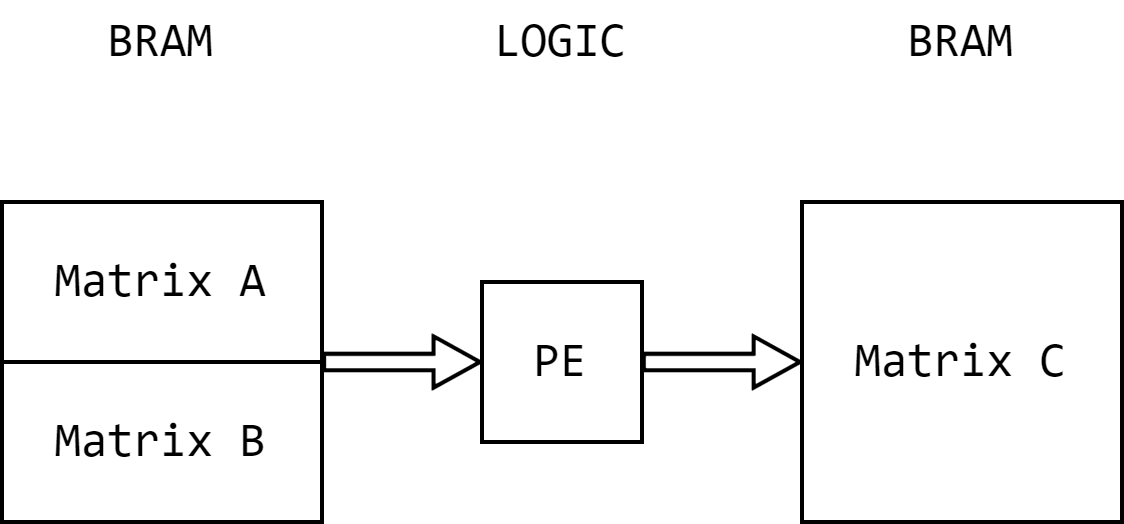
\includegraphics[width=0.5\textwidth]{lab4/1.png}
\end{figure}

\subsection{数据存储}
在本实验中,矩阵在BRAM中的存储方式为\textbf{行优先存储},与C/C++中的行为一致。在行优先存储模式下,矩阵的元素按照行的顺序依次存储在BRAM中。这意味着矩阵的每一行的元素都是依次排列的,然后再存储下一行的元素,以此类推。以矩阵$\boldsymbol{A}$为例,下图是行优先存储模式下矩阵$\boldsymbol{A}$在BRAM中的元素排列。

\begin{figure}[H]
    \centering
    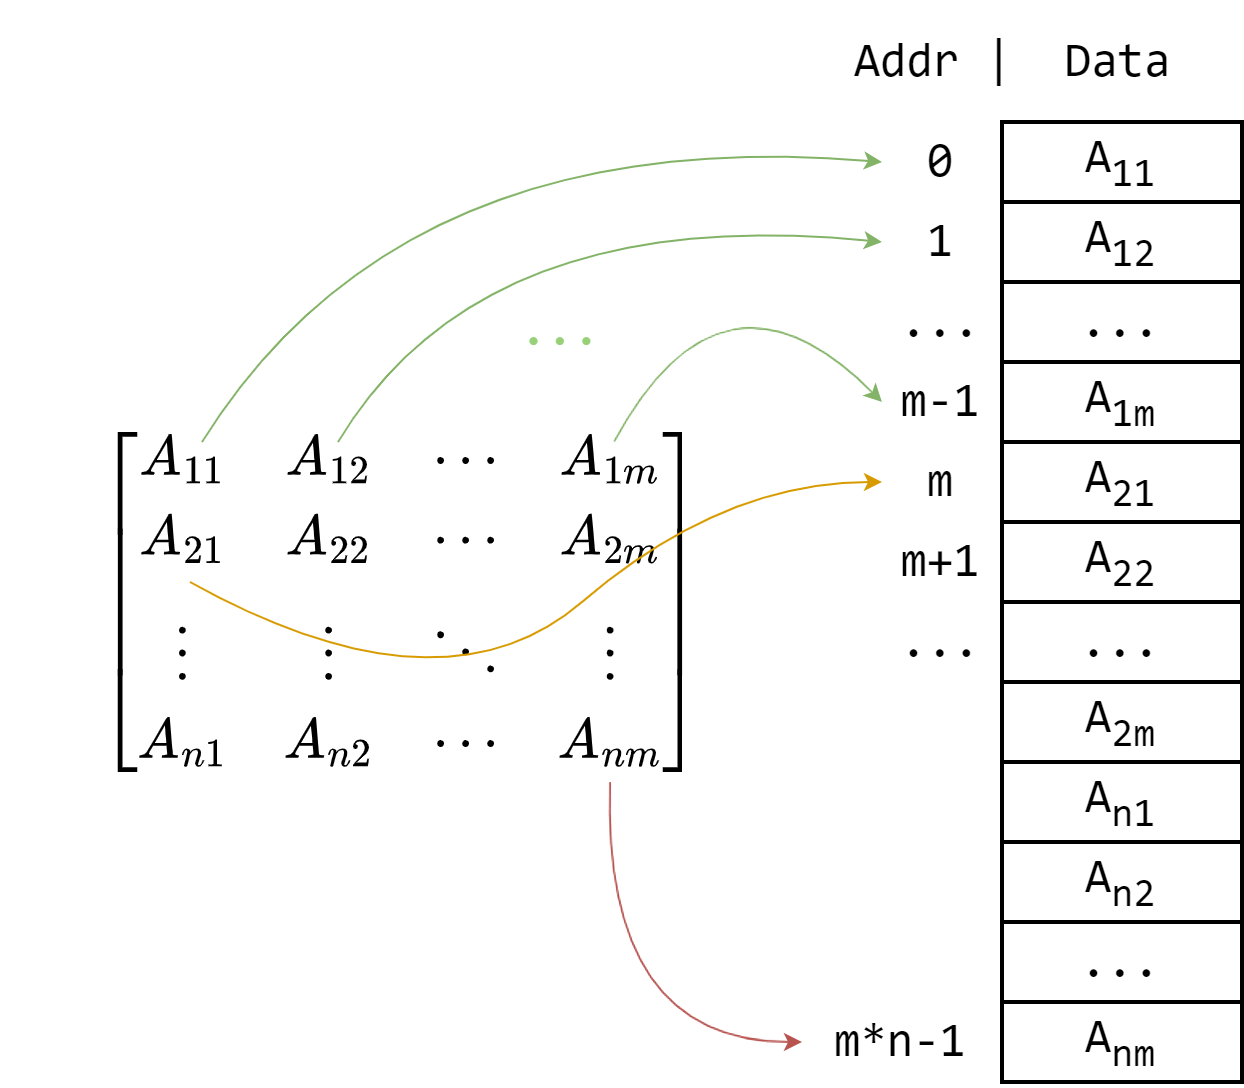
\includegraphics[width=0.5\textwidth]{lab4/2.png}
\end{figure}

在行优先存储模式下,矩阵元素位置的计算规则如下所示。

$$
Loc(A_{ij})=Loc(A_{11})+[(i-1)*m+(j-1)*1]
$$

在本实验中,矩阵$\boldsymbol{A}$与矩阵$\boldsymbol{B}$相邻存放在一块BRAM中,矩阵$\boldsymbol{A}$的元素存放在地址低位。在之前的实验中,我们已经学习了BRAM的基本使用方法。对于一个16*16维度的矩阵,存储其元素的BRAM的接口应如下图所示。

\begin{figure}[H]
    \centering
    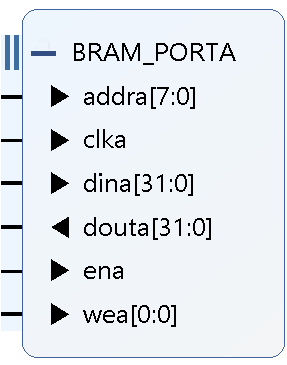
\includegraphics[width=0.2\textwidth]{lab4/3.png}
\end{figure}

在本实验中,BRAM采用的操作模式为写优先模式,在时钟上升沿到来时写使能有效,BRAM的读端口会输出写入的新数据,如下图所示。

\begin{figure}[H]
    \centering
    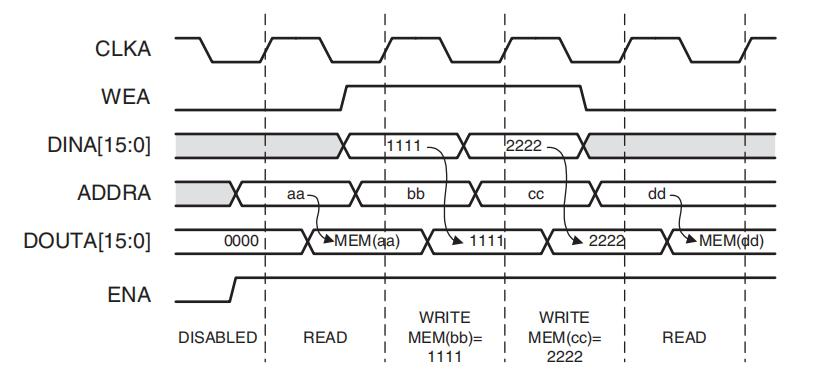
\includegraphics[width=0.8\textwidth]{lab4/4.jpg}
\end{figure}

\subsection{计算部件}
矩阵乘法会涉及到补码的乘法与加法,为降低设计难度,我们允许直接在Verilog代码中使用“ * ”与“ + ”操作符来实现乘法与加法操作。在先进的FPGA的EDA中,如Vivado,对Verilog代码中的“ * ”或“ + ”操作符,选择使用数字信号处理引擎进行实现,或选择使用可编程逻辑资源组成的快速进位链电路进行实现。对于两个32位补码的乘法,其逻辑框图如下所示(假设计算结果取低32位)。

\begin{figure}[H]
    \centering
    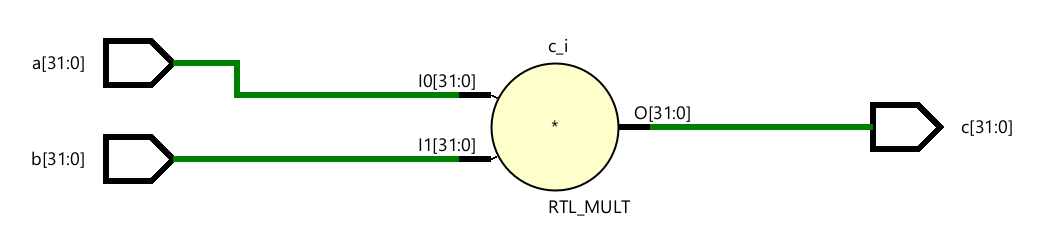
\includegraphics[width=0.8\textwidth]{lab4/5.png}
\end{figure}

在Vivado中综合后,可以看出,Vivado使用4个DSP48E1以实现该乘法操作,其电路图如下所示。

\begin{figure}[H]
    \centering
    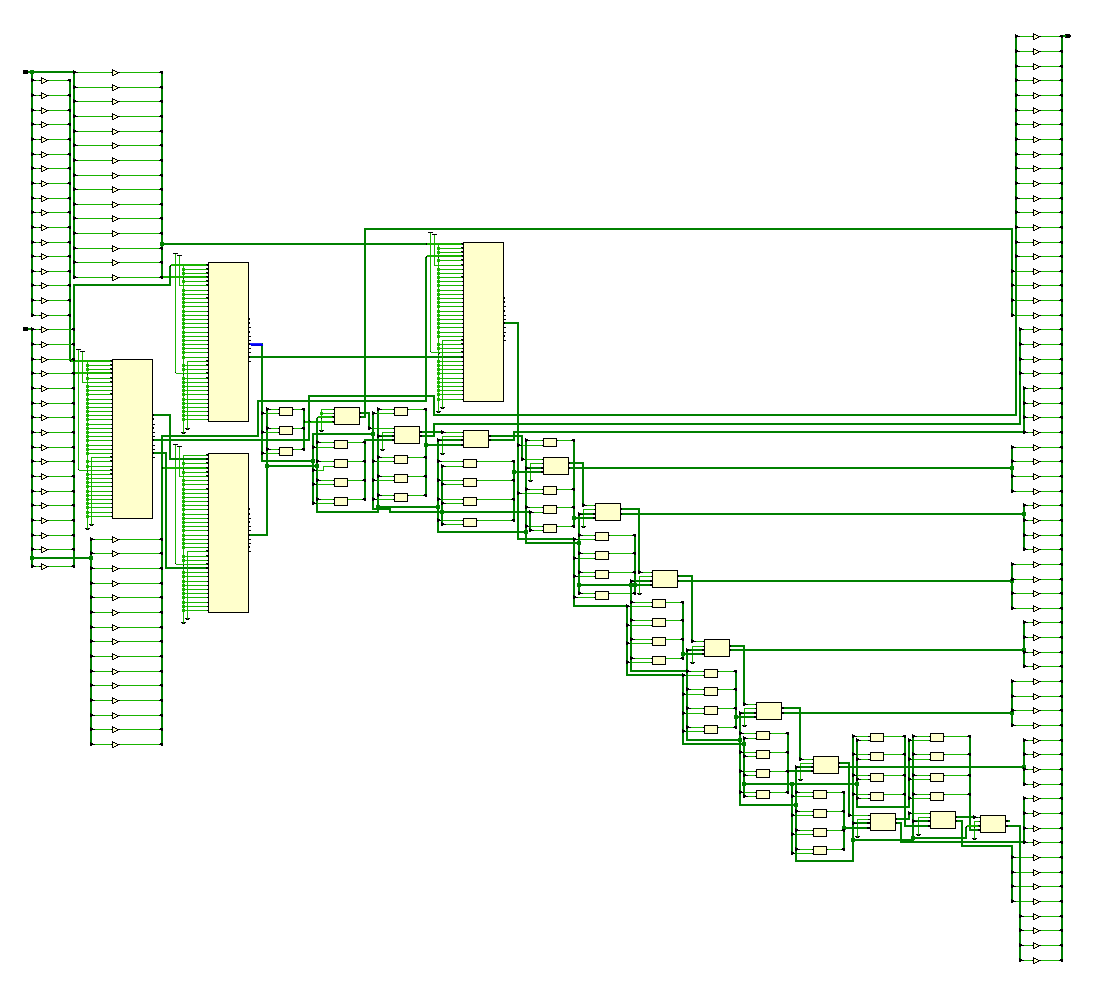
\includegraphics[width=0.8\textwidth]{lab4/6.png}
\end{figure}

\subsection{两个设计案例}

下面我们介绍两种极端设计案例,我们\textbf{不推荐}在您的设计中采用这种方法。第一种方法的整体架构如图所示。

\begin{figure}[H]
    \centering
    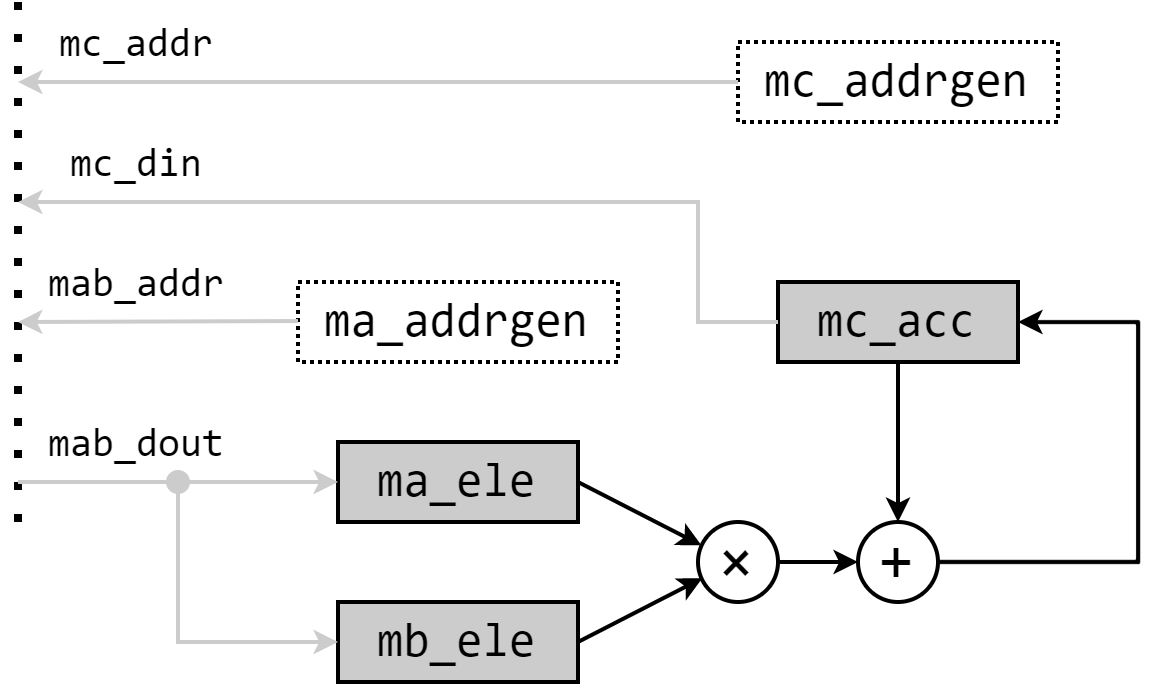
\includegraphics[width=0.5\textwidth]{lab4/7.png}
\end{figure}

其设计思路是,处理单元每次从矩阵$\boldsymbol{A}$的一行与矩阵$\boldsymbol{B}$的一列中各读出一个元素“ma\_ele”与“mb\_ele”,相乘后得到矩阵$\boldsymbol{C}$中一个元素的部分和,将部分和与寄存器“mc\_acc”中的累加值相加并暂存。接着处理单元继续从矩阵$\boldsymbol{A}$与矩阵$\boldsymbol{B}$中读出元素,直至矩阵$\boldsymbol{C}$的该元素计算完成,将结果写入BRAM。图中所示的地址生成单元使用状态机实现,用于生成矩阵A和矩阵B的读地址,以及矩阵C的写地址。

上述设计方法可以看作是C语言代码顺序执行的模拟,这样做并没有发掘FPGA的并行性。在同等工艺水平下,FPGA中的处理单元主频远小于CPU的主频,在FPGA上使用上述方法计算矩阵乘法,执行时间必定比CPU长。其次,上述设计方法没有进行\textbf{数据复用}。比如,在计算元素$AB_{11}$与$AB_{12}$时,需要重复读取向量$A_{1j}(j=1,2,...,m)$的值,造成性能下降,如下图所示。

\begin{figure}[H]
    \centering
    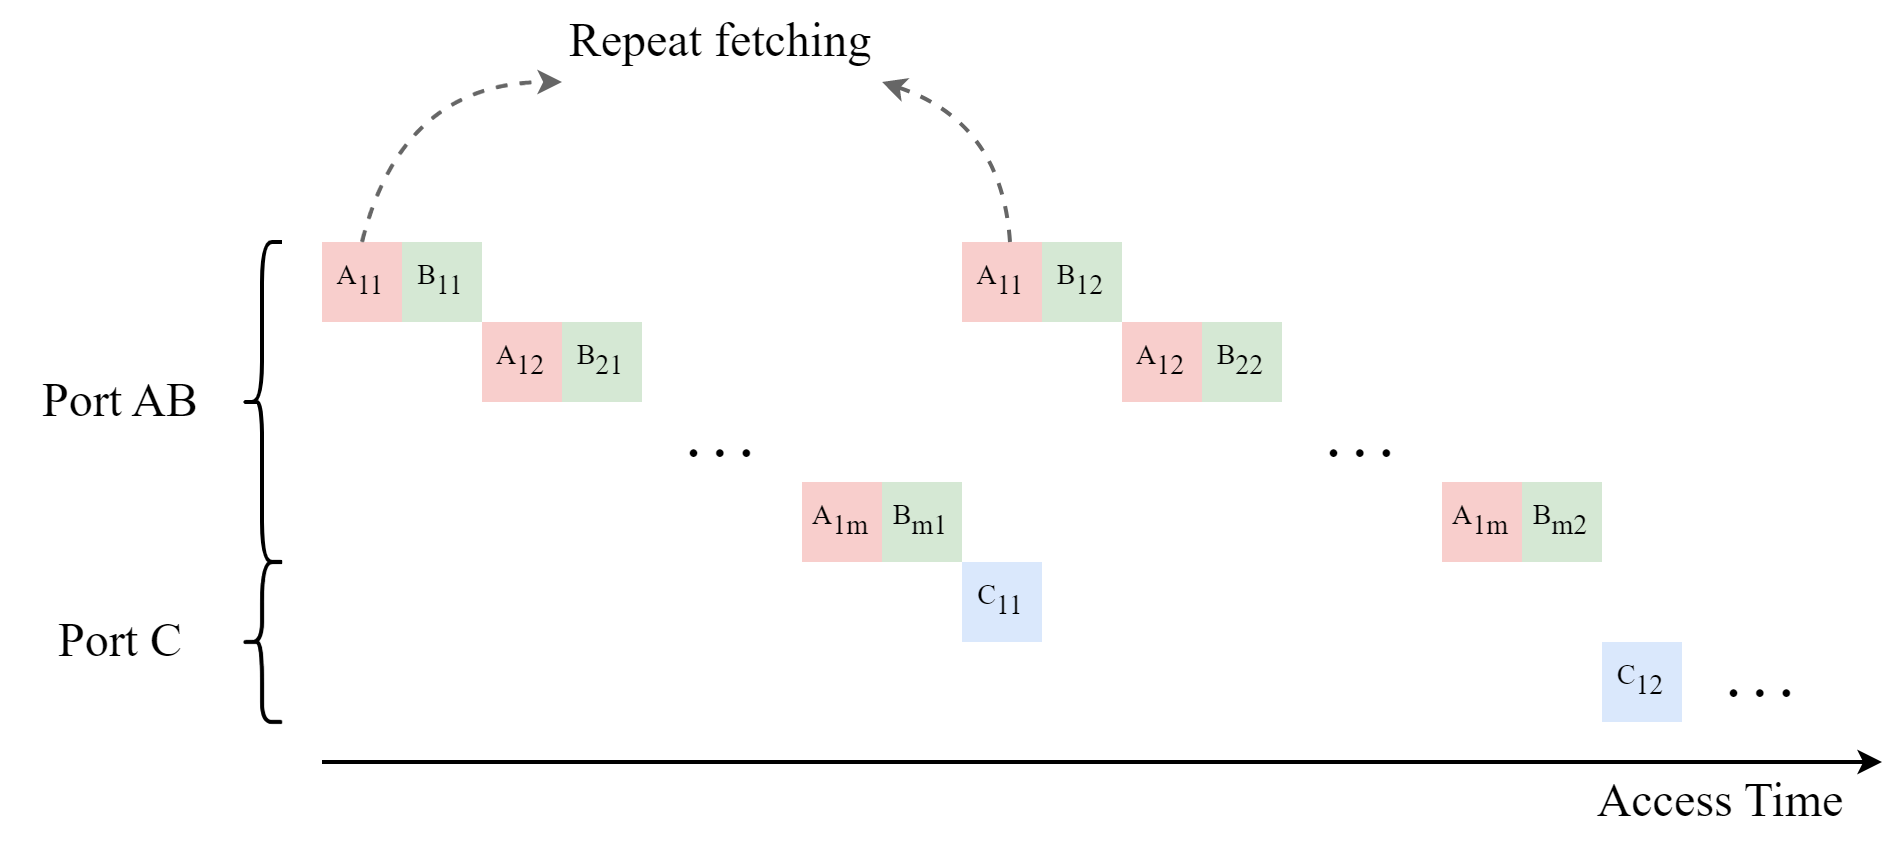
\includegraphics[width=0.8\textwidth]{lab4/12.png}
\end{figure}

第二种方法的设计思路是,将矩阵$\boldsymbol{A}$与矩阵$\boldsymbol{B}$中的所有元素读入处理单元并暂存,使用组合逻辑将三个循环展开以并行计算结果。该方法的示意代码如下。

\begin{lstlisting}[language=Verilog]
always @(*) begin
    for (n = 0; n < N; n = n + 1) begin
        for (p = 0; p < P; p = p + 1) begin
            c[n*N+p] = 32'b0;
            for (m = 0; m < M; m = m + 1) begin
                c[n*N+p] = c[n*N+p] + a[n*N+m] * b[m*M+p];
            end
        end
    end
end
\end{lstlisting}

由于处理单元需要同时计算多个结果,因此需要使用大量数字信号处理引擎与逻辑资源来实现多个乘法器和加法器。下图为计算6*6维度矩阵乘法完全展开三个循环的资源消耗。

\begin{figure}[H]
    \centering
    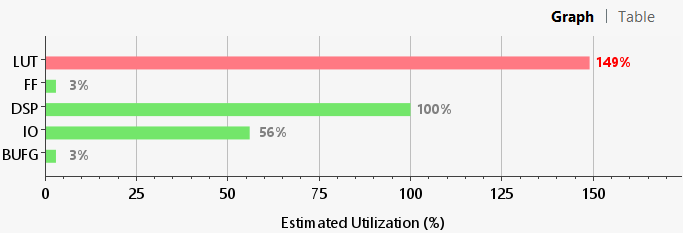
\includegraphics[width=0.8\textwidth]{lab4/8.png}
\end{figure}

\begin{figure}[H]
    \centering
    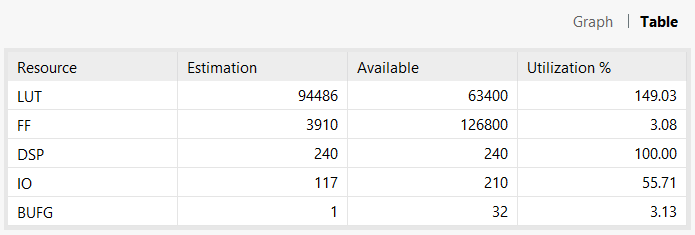
\includegraphics[width=0.8\textwidth]{lab4/9.png}
\end{figure}

从上图可以看出,器件xc7a100tcsg324-1上拥有240个数字信号处理引擎(DSP)资源。在数字信号处理引擎资源消耗完成后,需要使用逻辑资源(如LUT)来实现剩余的乘法器和加法器,造成了资源使用量溢出。

%------------------------------%

\section{设计要求}

本实验要求实现一个矩阵乘法处理单元,两个输入矩阵维度都是16*16,因此输出矩阵的维度也是16*16。所设计的矩阵乘法处理单元需要从提供的BRAM接口读取读取矩阵$\boldsymbol{A}$或矩阵$\boldsymbol{B}$的数据,完成计算后将数据从提供的BRAM接口写入矩阵$\boldsymbol{C}$的存储器。

本实验使用的FPGA器件型号为xc7a100tcsg324-1。本实验的要求为,在使用不超过器件上限的资源数量前提下,所设计矩阵乘法处理单元能在测试模块中运行通过。


\subsection{模块接口定义}

如下所示是矩阵乘法处理单元的模块接口定义,在“matmul.v”文件中已提供。模块从外部获取时钟信号与复位信号(高电平有效)。模块通过两个原生的BRAM接口访问矩阵的元素,操作模式为写优先模式。当所有计算完成且矩阵$\boldsymbol{C}$所有元素都被写入BRAM后,拉高ready信号以通知外部模块计算结束。

\begin{lstlisting}[language=Verilog]
module matmul(
    input           clk,
    input           rst,
    
    // matrix A & B access port
    output          mab_en,     // memory enable
    output          mab_we,     // memory write enable
    output  [ 8:0]  mab_addr,   // memory address
    input   [31:0]  mab_dout,   // memory read data
    output  [31:0]  mab_din,    // memory write data

    // matrix C access port
    output          mc_en,      // memory enable
    output          mc_we,      // memory write enable
    output  [ 7:0]  mc_addr,    // memory address
    input   [31:0]  mc_dout,    // memory read data
    output  [31:0]  mc_din,     // memory write data

    // indicate the result is ready
    output          ready

);

    // put your code here.

endmodule
\end{lstlisting}

\subsection{模块测试方法}

在我们提供的Vivado工程中包含了一个测试文件“matmul\_tb.v”,用以测试所编写的矩阵乘法处理单元,在Vivado中执行行为仿真即可。测试文件主要包含两个功能:计算结果验证与性能测量。

测试模块会实例化2个BRAM用以存储三个矩阵的元素,并从外部文件中获取初始化的值。当ready信号被拉高后,测试模块会从外部文件中读取正确答案,并与BRAM中的用户输出进行逐一对比,对比完成后会在命令行中输出验证结果,如下图所示。

如果计算结果错误,测试模块会给出相应元素在BRAM中的地址,并给出相应的参考结果。

\begin{figure}[H]
    \centering
    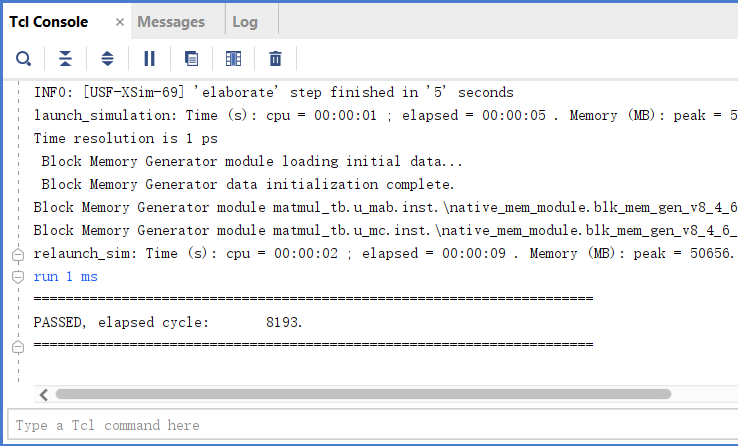
\includegraphics[width=0.8\textwidth]{lab4/13.png}
\end{figure}

\begin{figure}[H]
    \centering
    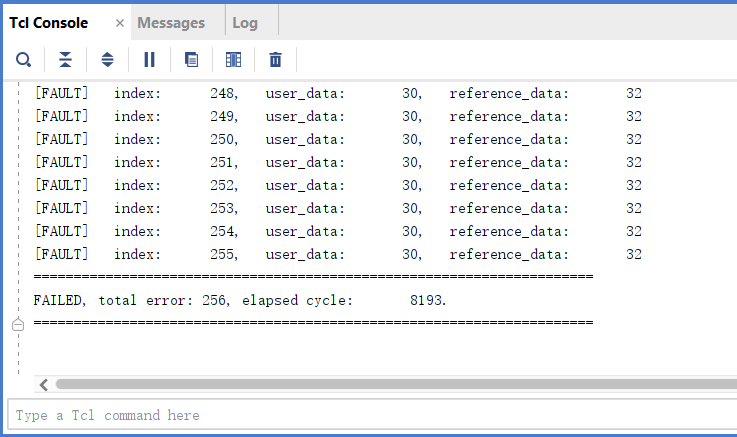
\includegraphics[width=0.8\textwidth]{lab4/14.png}
\end{figure}

测试模块还会测量您处理单元完成矩阵乘法计算所用的时钟周期,当然,这在计算结果正确的前提下才有意义。

\subsection{报告内容要求}

\begin{itemize}
    \item 您的处理单元设计方法
    \item 测试结果
    \item 综合后的资源使用情况表
\end{itemize}

%------------------------------%

\section{前沿方法(可选)}

目前的AI加速器和通用图像处理单元中会集成大量的矩阵乘法硬件单元以加速计算,它们大多数采用类似\textbf{乘加树}或\textbf{脉动阵列}的计算结构。如果您对这部分内容感兴趣,可以根据给出的参考文献,在您的处理单元中加入这些结构。

\subsection{乘加树}

乘加树即计算向量内积的计算单元,由$n$个乘法器以及$\lceil \log_{2}{n} \rceil$层的加法树构成,其结构如下图所示。

\begin{figure}[H]
    \centering
    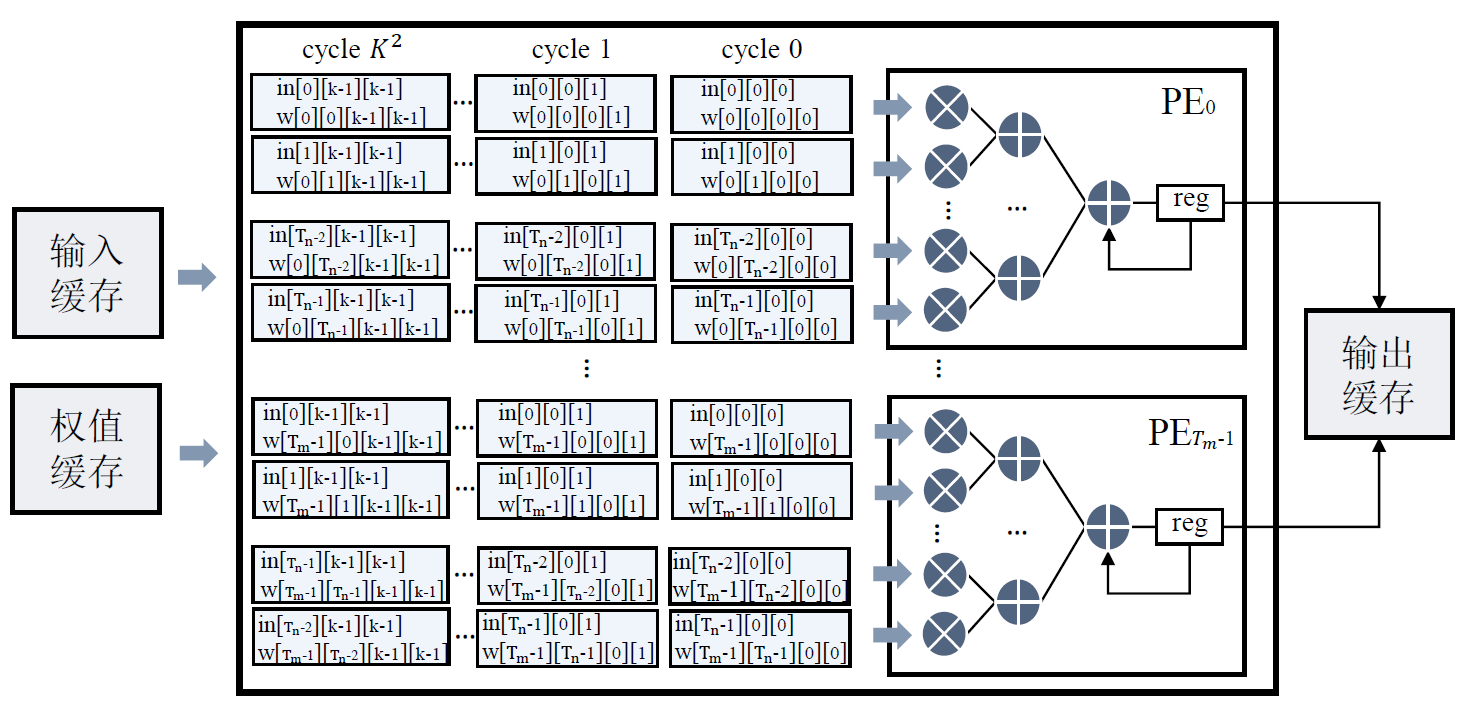
\includegraphics[width=0.8\textwidth]{lab4/10.png}
\end{figure}

乘加树结构在寒武纪的AI加速器中有大量应用,参考文献如下。

\begin{itemize}
    \item Chen T, Du Z, Sun N, et al. Diannao: A small-footprint high-throughput accelerator for ubiquitous machine-learning[J]. ACM SIGARCH Computer Architecture News, 2014, 42(1): 269-284.
    \item Chen Y, Luo T, Liu S, et al. Dadiannao: A machine-learning supercomputer[C]//2014 47th Annual IEEE/ACM International Symposium on Microarchitecture. IEEE, 2014: 609-622.
    \item Zhang S, Du Z, Zhang L, et al. Cambricon-X: An accelerator for sparse neural networks[C]//2016 49th Annual IEEE/ACM International Symposium on Microarchitecture (MICRO). IEEE, 2016: 1-12.
    \item Zhou X, Du Z, Guo Q, et al. Cambricon-S: Addressing irregularity in sparse neural networks through a cooperative software/hardware approach[C]//2018 51st Annual IEEE/ACM International Symposium on Microarchitecture (MICRO). IEEE, 2018: 15-28.
\end{itemize}

\subsection{脉动阵列}
脉动阵列是一种二维硬件结构,其基本组成单元是一个乘法器和累加寄存器组成的计算单元(MAC),MAC之间在水平和竖直方向上相互连接形成二维阵列。两个矩阵的输入数据从水平方向和竖直方向上流入,经过n个周期后在另一端得到计算结果,其结构如下图所示。

\begin{figure}[H]
    \centering
    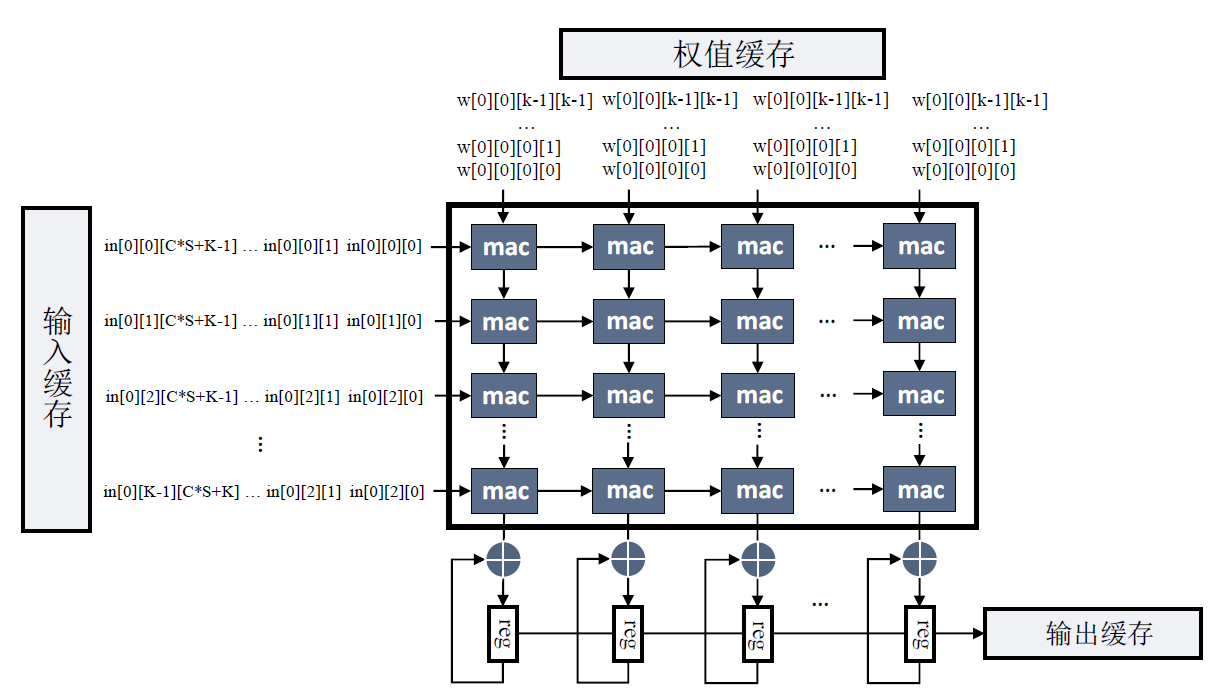
\includegraphics[width=0.8\textwidth]{lab4/11.png}
\end{figure}

脉动阵列结构在谷歌的TPU中有大量应用,参考文献如下。

\begin{itemize}
    \item Jouppi N P, Young C, Patil N, et al. In-datacenter performance analysis of a tensor processing unit[C]//Proceedings of the 44th annual international symposium on computer architecture. 2017: 1-12.
    \item Kung H T. Why systolic architectures?[J]. Computer, 1982, 15(1): 37-46.
    \item Lecture 8: https://www.cs.hmc.edu/courses/2001/spring/cs156/slides.html
\end{itemize}

\end{document}